\section{Figures}
\label{sec:figures}
\subsection{Schematic of the system}
asd

\subsection{Plots of Time-Varying Signals}
\begin{figure}[h]
    \centering
    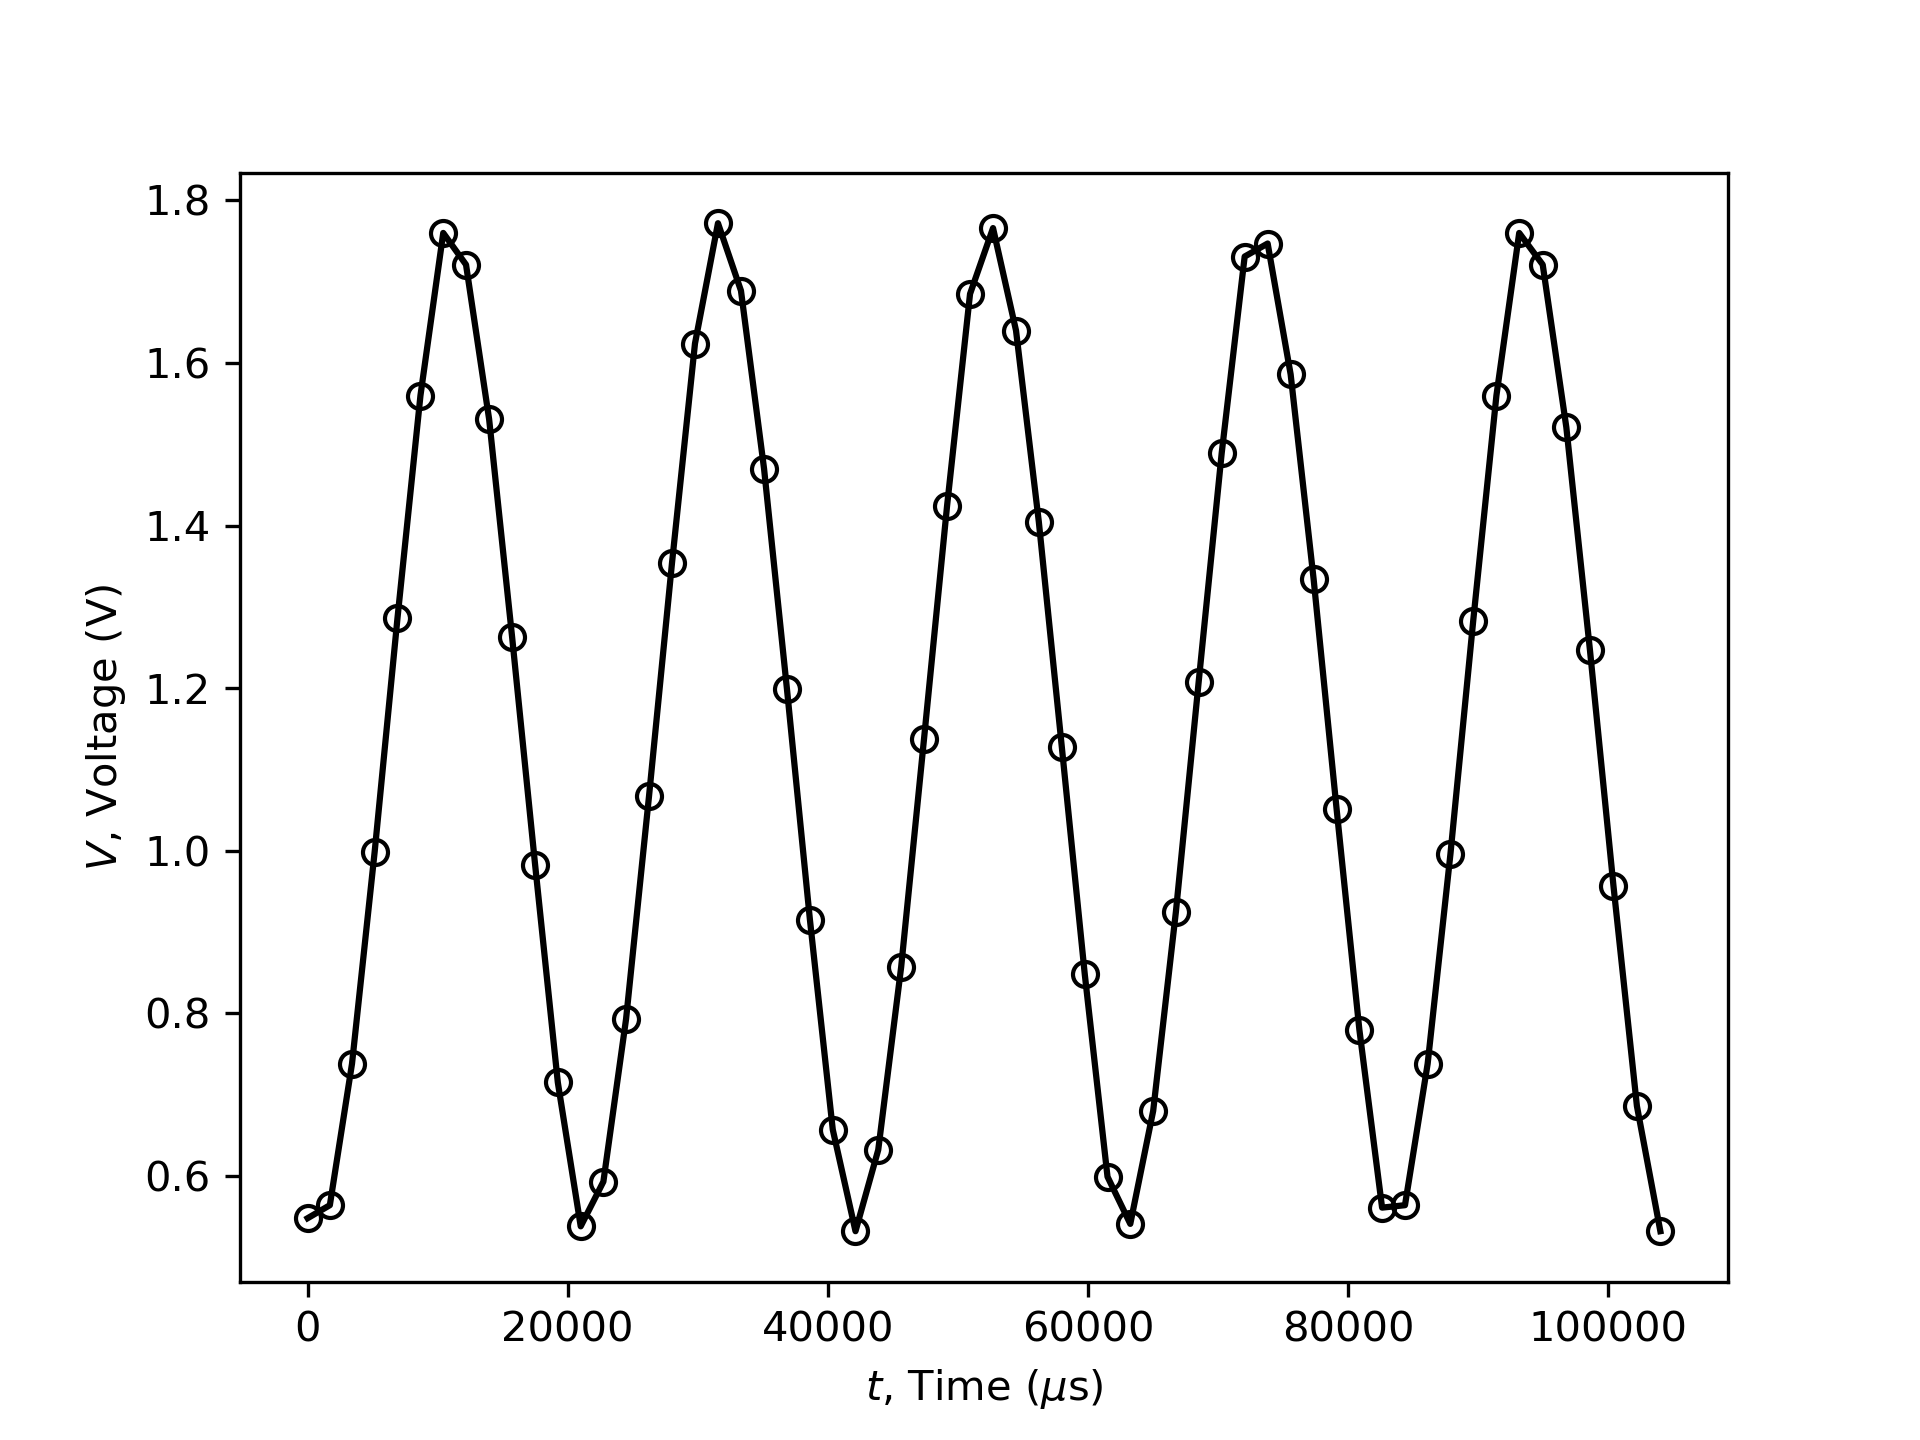
\includegraphics[width=0.5\textwidth]{Sections/Figures/10bit.png}
    \caption{Time varying signal of PCB 18 Measured with 10-bit ADC of the Arduino Uno}
    \label{fig:10bit}
\end{figure}

\begin{figure}[h]
    \centering
    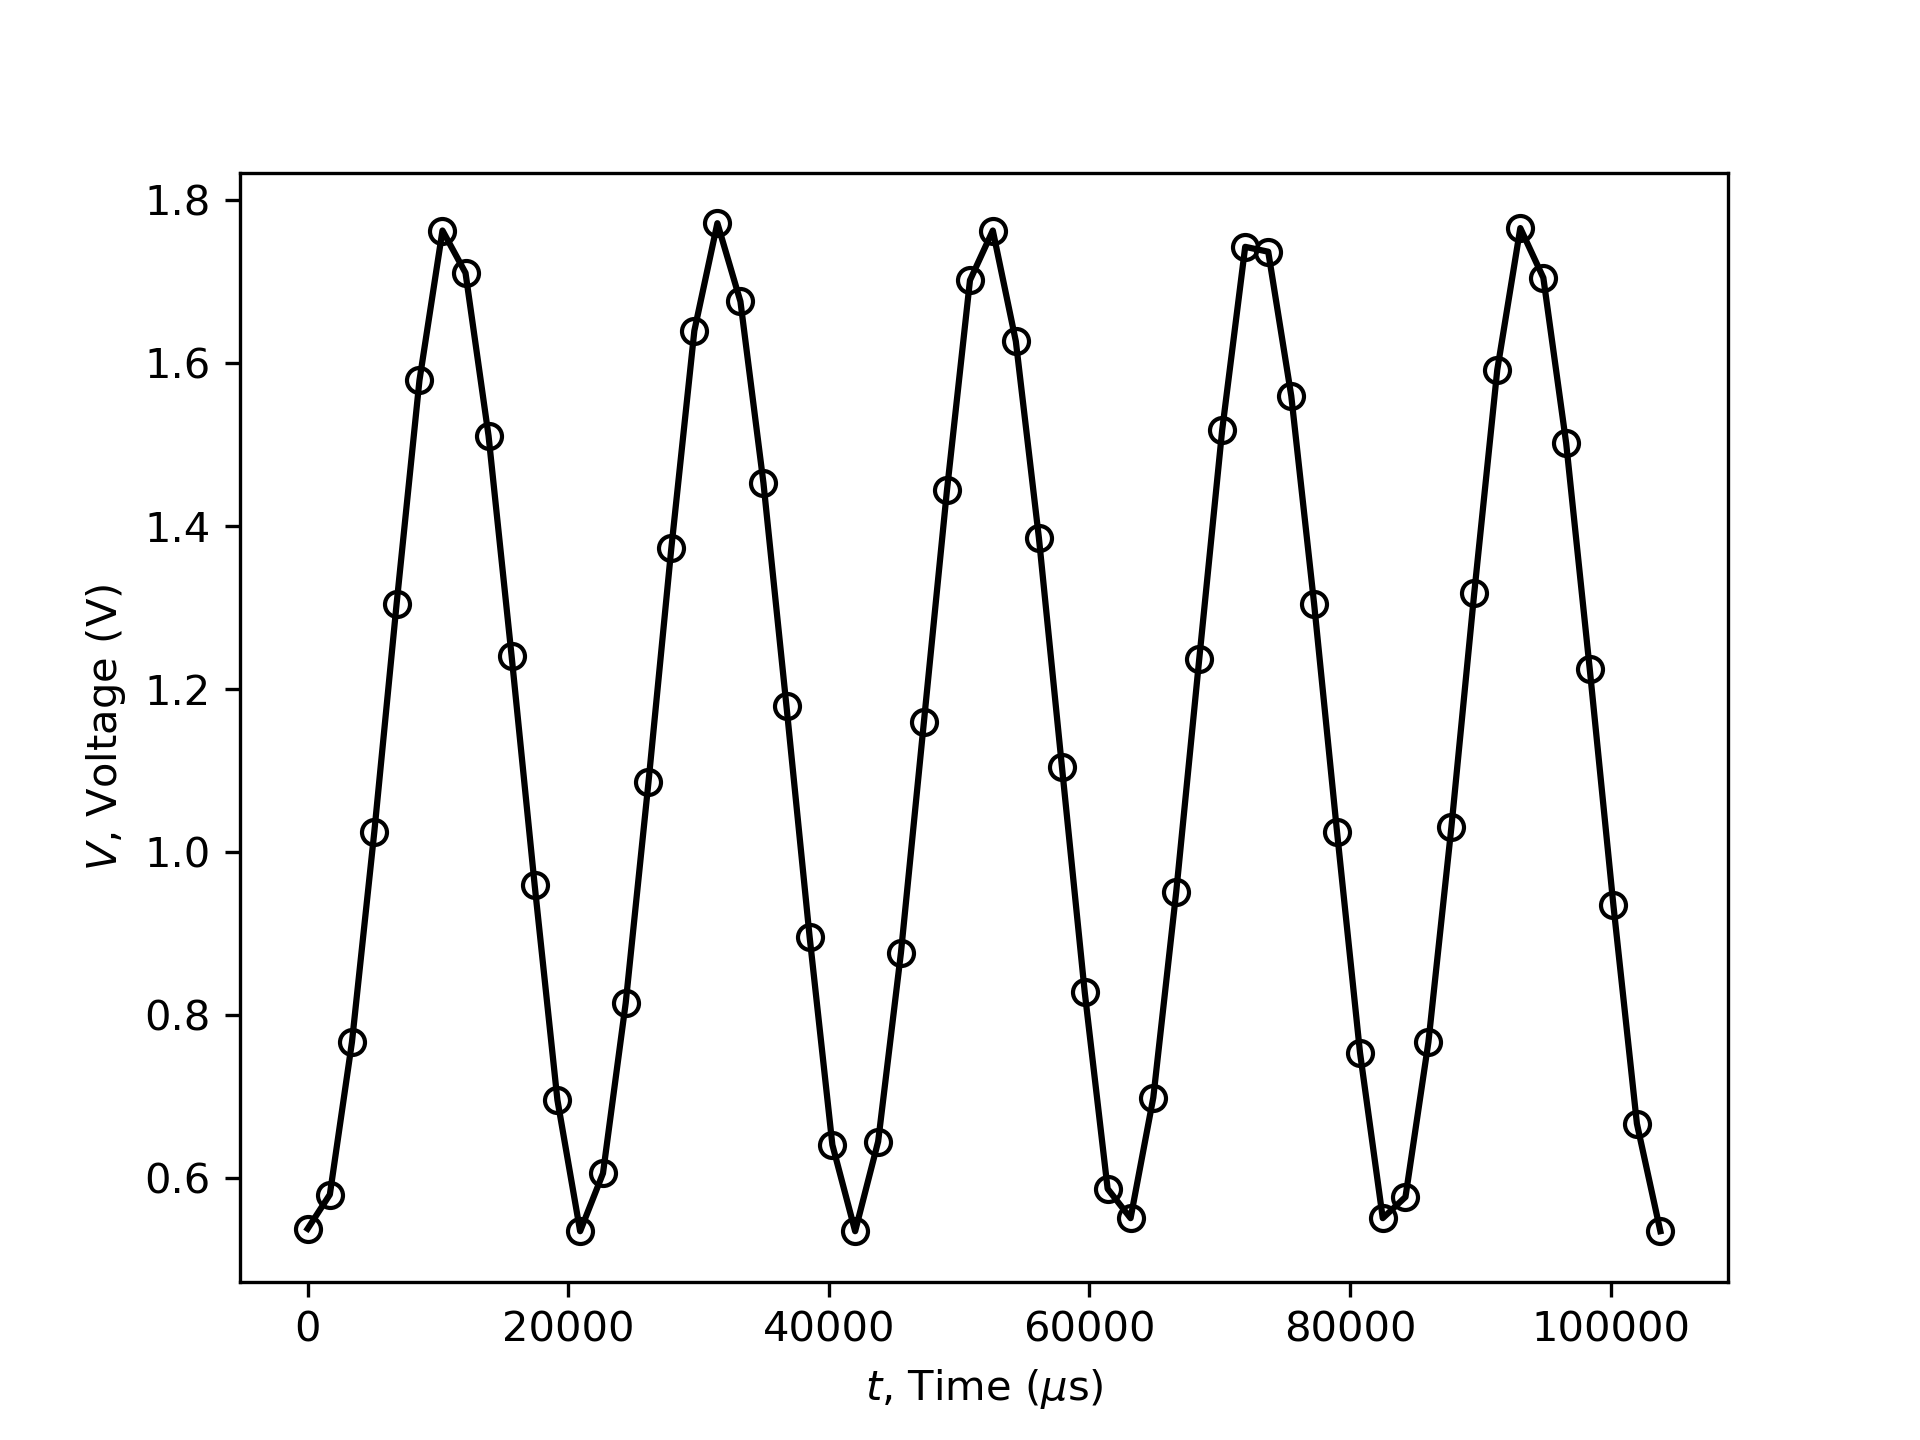
\includegraphics[width=0.5\textwidth]{Sections/Figures/5bit.png}
    \caption{Time varying signal of PCB 18 Measured with 5-bit ADC of the Arduino Uno}
    \label{fig:5bit}
\end{figure}